\documentclass[14pt,a4paper]{article}
\usepackage{txfonts}
\usepackage[utf8]{inputenc}
\usepackage[spanish]{babel}
\usepackage{amsmath}
\usepackage{amsfonts}
\usepackage{amssymb}
\usepackage{makeidx}
\usepackage{graphicx}
\usepackage{lmodern}
\usepackage{kpfonts}
\usepackage{fourier}
\usepackage{natbib}
\usepackage[left=2cm,right=2cm,top=2cm,bottom=2cm]{geometry}
\author{Rodriguez Lopez Francisco Javier}


\begin{document}
\begin{center}
\paragraph{\large UNIVERSIDAD POLITECNICA DE LA ZONA METROPOLITANA DE GUADALAJARA}


\includegraphics[width=6cm]{Upzmg.png} 
\end{center}
\begin{center}
\textbf{\LARGE Segundo Avance}\\
\end{center}
\begin{center}
\textbf{\LARGE Brazo Robótico}
\end{center}

\item \large Carrera: Ingeniería en Mecatrónica.\\

\item \large Curso: Sep-Dic 2019.\\

\item \large Fecha: 25 de octubre del 2019.\\

Docentes:\\

\item Morán Garabito Carlos Enrique.\\
\item Vázquez Alcaraz Laura Eugenia.}\\

\large{Integrantes:}\\
\begin{itemize}
\large{\item Cabrera Gutiérrez Raúl.
\item Gutiérrez Olivares Rogelio.
\item Guzmán Vázquez Jaime Alan Yamil.
\item Pérez de Alba Santiago Eduardo.
\item Ródriguez López Francisco Javier.
\item Romero Jauregui Osvaldo.
\end{itemize}

\newpage

\section{Titulo de Proyecto:}

Brazo robótico multidiplicinario con acoplamiento para diferentes tareas de grado industrial con libertad de movimiento y solución de problemas industriales.


\section{Planteamiento del problema:}

En contexto se presentara diferentes cuestiones que orientan a la realización del proyecto, por diferentes cuestiones los brazos robóticos son utiles y en el ambito empresarial estos son muy utilizados por su versatilidad y fácil manejo.\\
El brazo robótico tiene gran importancia en la industria, en general por esto se alenta a la realización de este, debido al grado de potencial que pueda tener, y puede ser maniobrado en diferentes ámbitos debido a su disposición y versatibilidad.\\
Las dificultades de este proyecto a futuro son cuestiones como el presupuesto, puede ser una de las mayor dificultades, a esto se le debe sumar cuestiones como la cotización de todos los materiales y precios para conseguir materiales de gran durabilidad.\\
En dificultades este tiene la compatibilidad con los diferentes accesorios para los que este pueda ser utilizado,  debido a los tipos de piezas empleadas para las diferentes cuestiones de la industria.\\
Estás dificultades son de gran importancia para este proyecto debido a que en cuestión de presupuesto o de inversión para el proyecto se necesitan piezas relativamente costosas debido a que se necesitan componentes de calidad para garantizar la cuestión de la durabilidad y eficiencia.\\
Para las dificultades anteriores se propone las distintas soluciones para la cuestión del presupuesto la solución a esto sería abaratar costos al crear, por ejemplo la base de el brazo de materiales reciclados o cuestiones similares además de tener una planificación en cuestión del presupuesto con un ingreso a plazos, como el proyecto esta basado a un año la administración de este, esto se debe solventar el problema del presupuesto.\\
Para que el problema pueda ser resuelto, la compatibilidad con las piezas de otros fabricantes, se implementara un sistema de intercambio de cabezales para lograr que el brazo robótico pueda ser compatible con estas diferentes piezas ádemas de la generacion de acoplamientos o adaptadores para el brazo robótico. \\
Las diferencias que se encuentran en el campo industrial que se pueden hallar en el proyecto, es completamente hecho con componentes comerciales mientras que los brazos robóticos industriales estan generados a mucho mayor costo ádemas de componentes de grado industrial y de mayor durabilidad y calidad, sin embargo este proyecto puede ser tomado a manera de prototipo podría ser llevado a gran escala.\\
El sustento en el que se basan los datos anteriores, se basara en el mercado actual así como los datos que se obtendran del mercado al igual que el funcionamiento de estos y los componentes en estimados asi como su precio en diferentes tiendas, así como en línea.\\
Los puntos anteriores esta basados en conocimientos adquiridos mediante el estudio de la implementación de estos en los medios industriales, al igual que el funcionamiento de estos fueron previamente estudiados.

\section{Formulación de Problema:}

En este apartado, se estaran viendo las preguntas que se puedan generar respecto a un futuro, dentro del proyecto:\\

¿Es buena idea suplementar esté tipo de dispositivos para otras actividades ademas del personal humano?\\
¿El brazo es algo eficiente a la hora de realizar su tarea?\\
¿Se puede, implemetar para tareas complejas que sean de eficiencia y rapidez?\\
¿Es buena idea de la implementación de automatización con esté tipo de dispositivos? 

\section{Objetivo General:}

Creación de un brazo robótico con la finalidad de adaptación a tareas complejas que el personal humano no realice con exactitud, mediante los conocimientos adquiridos y la demostración de habilidades y aptitudes que se tengan. 

\section{Objetivos del Proyecto:}

\begin{itemize}
\item Analizar y describir el buen funcionamiento del brazo robótico.
\item Empliamiento de tareas de aumatización.
\item Diseñar un modelo eficiente que capacite y proponga formas de adaptación a tareas humanas.
\item Demostrar los conocimientos que se adquieran, en los cursos. 
\end{itemize}

\section{Justificación:}

El brazo robótico, es una herramienta eficiente para ambientes, insutria-empresariales, para función y mejora del trabajo del personal común, que mejora la rapidez, fluidez y sustentación del trabajo a realizar, o en este caso alguna tarea en particular. El brazo robótico suplementa en eficiencia las tareas del humano, al fin de remplazar la lentitud y errores que este tiene.\\
El proyecto planteado en síntesis, tiene como idea, el  poder suplementar esas tareas empresariales que cuesta mucho dinero, energía y trabajo en cuestión, tratando complejos casos como la falta de personal, siendo este la sustitución perfecta para las manos laborales ordinarias, ambientado en el sector de automatización, y robótica, el cual pueda tambien agarrar temas, de control, y sustentación de las herramientas que se utilizaran en este proyecto, que en relevancia se adapte tanto al equipo como conocimiento, a la sociedad uan herramienta que pueda ser mejor innovada y utilizada, en otros campos.\\
Estructurado en primera instancia a la industria, la mecatrónica y sus amplias gamas de estudió que puede cubrir para la mejoración e implemetación, en las tareas que este pueda realizar, siendo varias y de ello, poder visulalizar en que constancia esté dispositivo esté apto para temas de mayor complejidad, viendo problemáticas que este tiene, a la  hora de implementarlos el sector de automatización, y las ganancias mismas de este.

\section{Limitación:}
Las limitaciones mas evidentes de este proyecto se deben a cuestiones como el límite de peso que soportara en carga, puesto que los materiales, los componentes así como la estructura general de este va estar diseñada para contener cierta capacidad de carga que sería en un rango entre los 400 g y los 700 g, limitandose a está, reiterando debido a cuestiones básicas de presupuesto ádemas de conocimientos debido al ciclo de formación intermedio, durante la ingeniería que limita el uso de algunas herramientas que más tarde se ven planteadas a ser utilizada, puesto que esté proyecto sera retomado para el último ciclo de formación en donde se actualizaran materiales y estructuras, así como componentes para mejorarlo, abundando en esto otra de las limitantes podría ser el precio de los componentes en general ya que es bien sabido que a mayor calidad mayor son los costos involucrados, en la elaboración de este, puesto al tamaño del proyecto asi como las restricciones economicas que se tienen.\\
Las dimensiones de este se toman como otra limitante, ya que por supuesto limitan la cantidad de peso que puede ser soportado así como la maniobrabilidad de este, y por defecto la resistencia, y eficiencia del brazo serian limitantes de rango alto.\\
Otras cuestiones que limitan de forma grande al proyecto se debe a la cuestion de base con la que este cuenta, es decir el proposito al que se quiere llegar y como esto cierra el camino hacia otras posibilidades, se optara por la realizacion de esté proyecto lo mas universal, que se pueda utilizar en diferentes ambitos sin que su contrucción pueda ser una limitante, sin embargo cuestiones como temperatura, humedad, entre otros factores climaticos, son limitantes a tener en cuenta, ya que la durabilidad de las tarjetas electronicas usadas, es menor que el resto del mecanismo empleado para este brazo robótico.

\section{Delimitación:}

Las delimitaciones en las que se enfocara, seran en mayor parte la eficiencia del brazo robótico, a la hora de mostrar el buen funcionamiento de este.\\
El área a centrarse, a partir de dicho planteamiento, y limitantes, es en la especificación de los grados de liberación que este brazo pueda tener, ádemas de cuanto es el peso que este pueda sostener, y por cuanto tiempo puede hacerlo, optimizando el trabajo mecánico que realizaría dicho dispositivo, a fin de centrarse en otros temas, como la velocidad en que realiza dichas tareas, asi como la complejidad o la fluidez en las que hace realiza dichas tareas.\\
Al fin de ver las fronteras de tiempo y espacio, que el estudió pueda tener. En secciones muestrales en donde se específica de mejor forma cada elemento a estudiar y a delimitar, en cierta parte, desde el tema del peso, hasta el tema de cuanto es el alcance que este brazo pueda alcanzar, esto viendolo a muestreo, y en rasgos de prueba , dureza, firmeza, y cálculos físicos, el cual a partir de la dinámica del dispositivo, se pueda demostrar las áreas a mostrar mejoras, y limitantes en su conceptualización de lo que es el brazo robótico, siendo este una temática que se realizaría dentro del desarrollo del brazo y su analisis de estudió.

\section{Marco Teórico:}

\subsection{Robots:}
Robots are diverse bunch. Som walk around on their two, four, sic or more legs, while others can take to the skies. Som robots help physcian to do surgery inside your body; others toil away dirty factories. There are robots the size of a coin and robots bigger than a car. Some robots can make pancakes. Others can land on Mars.

\subsection{Robot Arm:} 
A robot arm is a type of robot consisting of parts linked together in the same way as those of a human arm, monted on a stand.
The most common manufacturing robot is the robot arm which is usually made up of several metal segments.
Sensors were fixed to the robot arm to detect whether there were humans close to the robot.
A robot arm is a type of robot consisting of parts linked together in the same way those of a human arm, mounted on stand \citep{schilling1990fundamentals} .


\newpage

\section{Desarrollo:}

\section{Aportacion a cada Materia:}

\begin{tabular}{|p{70mm}|p{70mm}|} 

\hline
	MATERIAS & APORTACIONES ESPERADAS\\
\hline
	INGLES & La materia de ingles es importante puesto que toda la programación se realizara en ingles al igual que las fuentes de informacion consultadas.\\
\hline
	SISTEMAS ELECTRÓNICOS DE INTERFAZ & Esta materia ayudara a generar los conocimientos para realizar la fuente de voltaje que necesita el proyecto\\
\hline
	PROGRAMACIÓN DE PERIFÉRICOS & Los conocimientos de la programación del brazo se originan de esta materia.\\
\hline
	CONTROLADORES LÓGICOS PROGRAMABLES & La aportación de esta materia sería el grafcet para la  programacion del proyecto\\
\hline
	ESTRUCTURA Y PROPIEDADES DE LOS MATERIALES & normas de seguridad como selección de materiales para estructura\\
\hline
	ÉTICA PROFESIONAL & Resonsabilidad y seguimiento de normas al momento de realizar las evidencias del proyecto ádemas  de dar seguimiento a los códigos establecidos para la ingeniería.\\
\hline
\end{tabular}\\\\


\begin{tabular}{|p{70mm}|p{70mm}|} 

\hline
	MATERIAS & APORTACIONES REALIZADAS\\
\hline
	INGLES & Se consultaron fuentes de información en ingles para la realización de los circuitos y programación.\\
\hline
	SISTEMAS ELECTRÓNICOS DE INTERFAZ & Se aplican los diferentes componentes vistos en la materia para realizar la fuente de voltaje variable.\\
\hline
	PROGRAMACIÓN DE PERIFERICOS & Se utiliza phyton y su generación de interfaz para el control del brazo.\\
\hline
	CONTROLADORES LÓGICOS PROGRAMABLES & Se diseña el grafcet para la mejor estructuración de la programación.\\
\hline
	ESTRUCTURA Y PROPIEDADES DE LOS MATERIALES & Se investigan los diferentes posibles materiales para la estructura del proyecto de acuerdo a sus propiedades.  \\
\hline
	ÉTICA PROFESIONAL & Se siguen los comportamientos éticos durante el proceso de realización del proyecto como podria ser la autonomia del profesionista, ademas de atender al código profesional de ingenierías.  \\
\hline
\end{tabular}


\section{Diagramas:}

\begin{center}
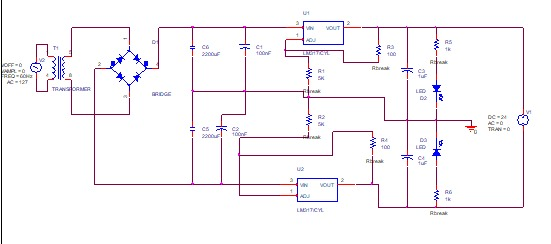
\includegraphics[width=12cm]{Fuente.jpeg} 
\end{center}

En el diagrama de la fuente de alimentación regulada, se verán los componentes que esta tendrá, siendo el más destacado de ello el regulador de voltaje líneal Lm317, se propuso este componente, como una estimación de lo que otros componentes podrían también hacer, como lo es regular el voltaje y variarlo al valor que se ocupe (En esté caso para los motores), pero esto se estimara de mejor forma, ya que entremos a temas de convertidores de voltaje, en la clase de Sistemas Electrónicos de Interfaz. Por esta parte adquiriendo el conocimiento suficiente para poder establecer un mejor componente, o un mejor acomodo del esquématico,para mejoras e innovaciones que podría tener el sintetizar este tipo de fuentes para el uso en el trabajo mecánico, en cuestion de potencia. En este se toma en cuenta que el voltaje mínimo que puede manejar son 1,25v a 100mA, especificaciones que son de ayuda.\\

Nota: En la parte, de la transformación, se encuentra un panel de amperimetro/voltimetro, el cual no fue añadido a vista, dadas las faltas del saber del software, ádemas de la realización de regulación (Que puede ser modificada, al tener mejor y más apto conocimiento).

\section{Cálculos:}
En sección al cálculo del brazo robótico. Para poder empezar con el cálculo dinamico de esté brazo robótico, en constancia de previsualización a una estimación dadá hípotesis en perpectiva a los materiales y a la resistencia que tendran estos, para el movimiento, carga y distribución de peso de este, Siendo este caso, mas simplificado, para no atraer problemas a la hora del armado que tenga esté y sus piezas.\\

Características del brazo:\\
Altura: 40 cm apoximadamente.\\
Peso: 8Kg aproximadamente.\\
Características del motor:\\
Voltaje dc: 6v-24v.\\
Corriente: 1.10 A.\\
Revoluciones: 10,000rpm.\\
Diámetro del motor: 36mm.\\
Diámetro del torque: 3.17mm.\\
Con esas características, se puede dar una idea, de como quedaría establecido la dinámica del brazo robótico, en este caso, viendo más que nada factores como los motores, o el peso que cargara el brazo y en estancia con que esfuerzo.\\
Se calcula de primera estancia el trabajo de los motores, estabeciendo el trabajo de estos:\\

Establecemos el punto de partida de la posición en la que se encontara al momento del giro del motor:\\

$$ \emptyset=\frac{4mm}{3.17mm}= 1.3mm $$

En constancia al centro del diámetro, el momento en que se mueve este, se encontrara en 1.3mm, respectivamente en movimiento.\\
Ahora queremos cambiar de revoluciones, a radianes por segundo, para asi poder ver el movimiento en los 360°, que esta establecido el torque del motor, quedando:\\

$$ 1rev=2\pi=360°$$

$$ 10,000 \frac{vueltas}{min}*\dfrac{2\pi rad}{1 vuelta}*\frac{1 min}{60s}= 333.3 \pi rad/s $$

Simplificando \pi queda:\\

$$ 333.3 rd/s* \pi= 1,047.2 rd/s $$

Ahora teniendo datos, simplificados, para ver como trabajara en la realización mecanica, el motor, podremos calcular el momento, entre otros factores del brazo, para su péso en una previsualización.\\

$$ M= P*D $$

Simplificando datos:\\

$$ M=0.40m*8kg= 3.2 m/kg $$

Esto ayuda a la hora de carga del objeto en cuanto la garra, y el motor, simplificando el trabajo que pueda hacer tanto mecanico, como de potencia.\\
En otro punto, el centro de masas nos ayuda en este caso, a ver el estable movimiento en el que se puedan encontrar tanto el peso del brazo, como el del objeto a cargar, siendo este:\\

$$ CM=\frac{3.2 m/kg}{8kg}= 0.40m $$

Como se aprecia en el resultado, nos da el inicio del brazo, esto quiere decir que el centro de estabilidad, se encuentra al principio de este. Conceptuando la longitud que tendra el brazo, y donde tendra todo su ímpetu, a la hora de carga y de trabajo.\\
En otro caso, el trabajo que pueda realizar este, dejandolo con la siguiente fórmula:\\

$$ W= F*cos(45°)*d $$

Esta fórmula respectivamente del ángulo es un alcance del ángulo que puede tener para la liberación de grados de libertad.\\

$$ W= 160N*cos(45°)*0.40m= 48.7 J $$

Dejandonos apreciar el trabajo que se podría tener, en un punto del agarre.\\

Nota: Estos cálculos, solo son una perpectiva, de lo que podría ayudarnos, a terminos mas complejos, como el caso de las articulaciones, y el manejo de la potencia en conjunto, siendo estos una guía de poder ver la realización y el armado, de los motores respecto al centro de carga y el alcance que podría tener, este brazo robótico, analizandolo más adelante, con dinámica avanzada.\\

\textbf{Fuente de Alimentación Variable:\\}
Los cálculos de la fuente variable queda establecido en la visualización del esquemático:\\
La fórmula para la obtención del voltaje, dadás resietncias es:\\
$$ V_{out}= 1.25v(1+\frac{R1}{R2}) $$
Obteniendo datos:\\
$$ V_{out}= 1.25v(1+\frac{3900 ohm}{220 ohm})=23.4 voltios $$
Esta primera fórmula sintetiza, los valores de la resietncia R1 y R2, que nos ayudan a que el flujo de la corriente sea específico. Quedando el voltaje de salida en 23.4v.\\

$$ Vp= \frac{V_{rms}}{0.707} $$

Obteniendo datos:\\

$$ Vp=\frac{16v}{0.707}= 22.6 v $$

Está fórmula obtiene los datos, del Vrms, los 16v, son los del transformador que se podria utilizar. Ahora se aprecía en el esquemático, que hay un puente de diodos, conectando dos diodos, al transfromador y los otros tanto parte negativa, como parte positiva del Lm317 en el Vin, nos dejan un resultado de la siguiente forma:\\

$$ V_{dc}=\frac{2(22.6v)-1.4v}{\pi}= 14 v. $$

En esté cálculo, se tiene en cuenta que son dos diodos los que están trabajando sobre la misma entrada, por lo qué un solo diodo tiene 0.7v, esto multiplicado por dos sería 1.4v. En otro caso el dos que mutiplica al voltaje 22.6, es la cantidad de diodos que hay en ese punto.\\
Teniendo ya los voltajes, se saca la potencia con la que trabajaremos, en este caso, entre más potencia haya, menos ruído podra tener la regulación del voltaje, en este caso, siendo multiplicado por dos el voltaje del transformador, nos da un resultado de 32 Vatios. Ahora si sacamos la corriente establecida en el diagrama.\\

$$ P= (V)(I)= 32vatios=(22.6v)(I) $$

Sustituyendo la fórmula, para encontrar la corriente se hace un despeje:\\

$$ I= \frac{32va}{22.6v}= 1.4 A $$

Esté valor de corriente, establecida en todo el circuito es la indicada, para el buen torque de los motores, y el movimiento de estos.\\
Para el uso de los capacitores es bueno tener en cuenta de que valor y de que capacidad se tendrán que tener, para establecer un mejor flújo del voltaje. En los primeros dos capacitores son electroliticos, con un valor en Faradios de 2200uF a una capacidad de 30v, esto para que el voltaje que recae en las resistencias sea bien distribuido y no se sobrecargue el condensador.\\
Los segundos, son cerámicos, esto para que el flujo de corriente y el momento de carga sea mas pura, con un valor de 100nF a una capacidad de 50v, para que administre de mejor forma la regulación de voltaje y la tercera línea de capacitores es de 1uF a 30v, esto para lo mismo, que al momento de carga, no se desperdicie demasiado, y pueda salir el voltaje que se requiere, para el funcionamiento correcto de los motores.

\section{Diagrama de Gantt posibles Materiales y Gastos:}

\begin{center}
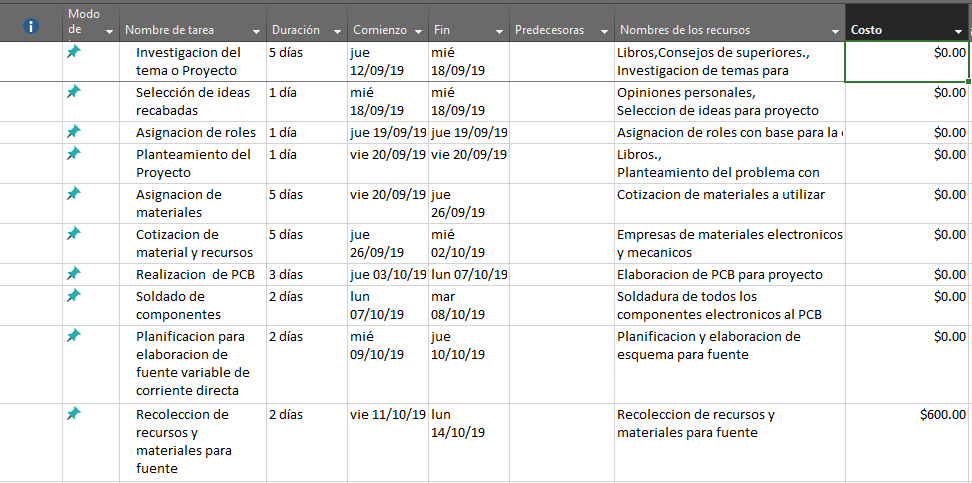
\includegraphics[width=15cm]{DefinicionTareas/4.png} 
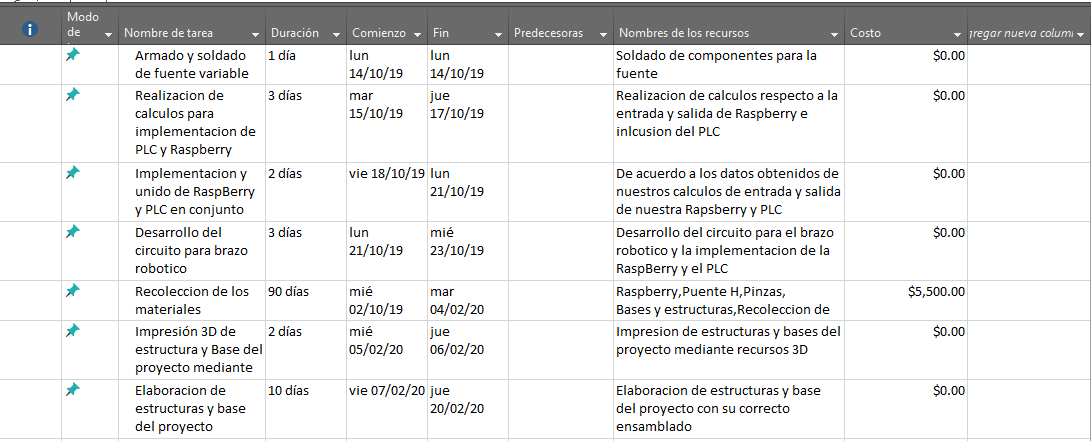
\includegraphics[width=15cm]{DefinicionTareas/5.png} 
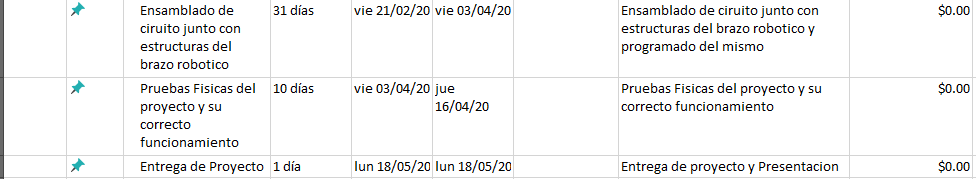
\includegraphics[width=15cm]{DefinicionTareas/6.png} 
\end{center}

\newpage
\section{Diagrama de Gantt Cronograma de Actividades y Tiempo:}
Cronograma de trabajo, fechas establecidas del 12 de  Septiembre del 2019 al dia de entrega, 18 de mayo del 2020

\begin{center}

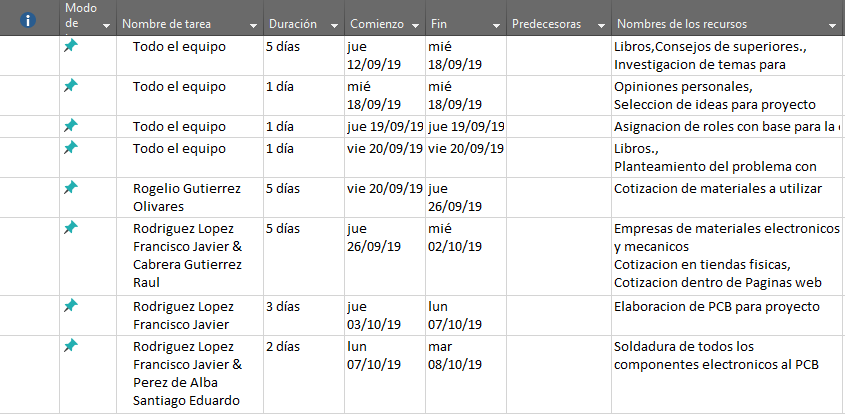
\includegraphics[width=13cm]{Esquema1.png} 
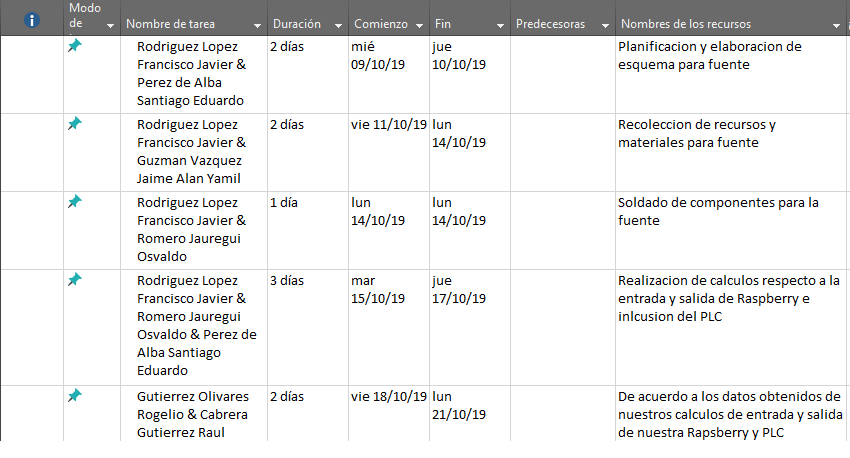
\includegraphics[width=13cm]{Esquema2.png} 
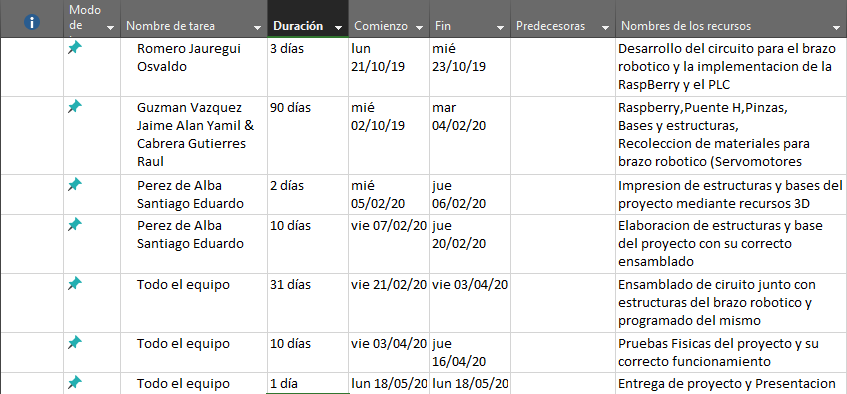
\includegraphics[width=13cm]{Esquema3.png} 

\end{center}

\section{Propuesta de Materiales:}

\subsection{Elementos consturctivos}
\begin{enumerate}
\item Manipulador o brazo mecanico.
\item Elementos motríces o actuadores.
\item Controlador.
\item Efector termínal.
\item Sensores de información.
\item Motor a Pasos.
\end{enumerate}

\subsection{Manipulador}
Es el conjunto de elementos mecanicos que permiten el movimiento del efector termina. En la estructura interna del manipulador se encuentran ubicador muchas veces los elementos motrices, engranajes y tranmisiones que soportan el movimiento de las cuatro partes, que por lo general conforman el manipulador, las cuales son \citep{puglisi2006protesis}:\\
1-Base o pedestal de fijacion.\\
2-Cuerpo.\\
3-Brazo.\\
4-Antebrazo.\\
\subsection{Elementos motrices o Actuadores}

\begin{itemize}
\item \textbf{Neumáticos}:
Emplean aire comprimido como fuente de energía y son adecuados en el control de movimientos rapidos, pero su precisión es limitada.\\
\item \textbf{Hidráulicos}:
Los actuadores hidráulicos son recomendables en los manipuladores que tiene una gran capacidad de carga, junto a una precisa regulación de velocidad \citep{turiel2002aplicaciones} .\\
\item \textbf{Electricos}:
Los motores eléctricos son los mas utilizados, gracias a su precisión y la facilidad de control.
\end{itemize}

\subsection{Controlador:}
Es el dispositivo encargado de regular el movimiento de todos los elementos del manipulador, y de realizar los cálculos y procesado de la información. La complejidad del control varia segun los parametros que se gobiernan \citep{cardenas2015diseno}.
\subsection{Efector Terminal:}
Es la garra o herramienta que se le acopla a la muñeca del manipulador, siendo el encargado de materializar el trabajo previsto por ejemplo, este puede ser una tenaza, un electroiman, o algún otro aparato. En general, y de acuerdo al tipo de aplicacion, la problematica del efector terminal radica en que este ha de posser una elevada capacidad de carga y al mismo tiempo es importante que tenga un peso y tamano reducido. Por esto, en muchas ocasiones es necesario disenar el efector terminal de acuerdo a los requerimientos de la aplicacion en que se utilizara.
\subsection{Sensores de Información:}
Los robot inteligentes son aquellos capaces e adaptarse al ambiente y tomar decisiones en tiempo real, adecuadas para situación. La información que ellos reciben les hace autoprogramables, es decir,alteran su actuar en función de la situación externa, lo que los hace poseer un cierto grado de inteligencia artíficial. A este respecto, las informaciones mas solicitadas por los robots son las que hacen referencia a la posición, velocidad, aceleración, fuerzas,pares, dimensiones y contornos de objetos, y temperatura.
\subsection{Motor a Pasos:}
\textbf{Funcionamiento:}\\
Este motor a pasos NEMA17 es bipolar, tiene un ángulo de paso de 1.8°(200 pasos por vuelta) y cada bobina es de 1.2A a 4V, capaz de cargar con 3.2kg/cm. Es un motor muy robusto ampliamente utilzado en impresoras 3D caseras.
\textbf{Características:}\\
Este motor cuenta con:\\
\begin{enumerate}
\item Tamano: 42.3*48mm, sin incluir el eje.
\item Peso: 350 gramos.
\item Diámetro del eje: 5mm.
\item Longitud del eje: 25mm.
\item Pasos: 200.
\item Corriente: 1.2 Amperios por bobinado.
\item Tensión: 4V.
\item Resistenica: 3.3 Ohm por bobina.
\item Torque: 3.2kg/cm.
\item Inductancia: 2.8 mH por bobina.
\end{enumerate}
\textbf{Aplicación:}\\
Los motores paso a paso se utilizan generalmente en una variedad de aplicaciones donde el control de posición exacta es deseable y el coste o la complejidad del sistema de control sea justificada.\\
\begin{enumerate}
\item Impresoras CNC.
\item Impresora 3D / prototipos de maquinas.
\item Cortadoras laser.
\item Actuadores lineales.
\item Discos duros .
\end{enumerate}

\section{Presupuesto:}

\begin{tabular}{|l|l|l|l|}
\hline
	Producto & Piezas & Precio & Total\\
\hline
	Impresión 3D & 5 & 70 & 350\\

\hline
	Capacitores 2200uF,1uF, 100nF & 3 & 5 & 15\\
\hline
	Regulador LM317 & 1 & 15 & 15\\
\hline
	Resistencias varias & 20 & 2 & 40\\
\hline
	Diodos1N4004G & 16 & 5 & 80\\
\hline
	1 Switch & 1 & 10 & 10\\

\hline
	Fuente CA-CD & 1 & 600 & 600\\
\hline
	Push bottons & 8 & 2 & 16\\
\hline
    Cautin & 1 & 150 & 150\\
\hline
	Estaño & 1 & 30 & 30\\
\hline
	Multimetro & 1 & 100 & 100\\
\hline
    Motores DC & 5 & 400 & 2000\\
\hline
\end{tabular}

\section{Prototipo y Simulacion:}
\begin{center}
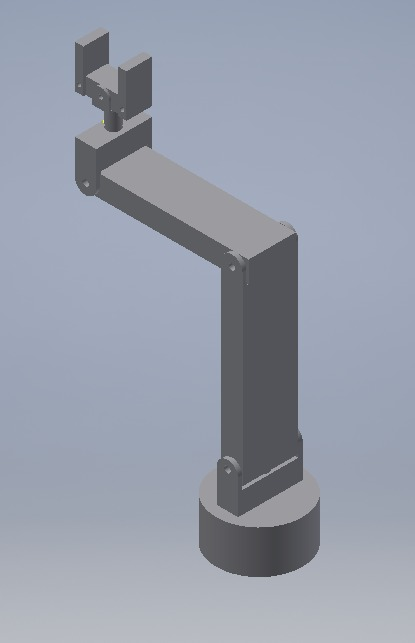
\includegraphics[width=6cm]{Proto.jpeg}
\end{center}

\newpage

\bibliographystyle{plain}
\bibliography{Ref}


\end{document}